\chapter{Experimental Evaluation}\label{chap:experiments}
This chapter will investigate the~performance of the~\emph{hybrid} approach for integrated synthesis methods extensions \,--\, multi-property and optimal synthesis \,--\, for various case studies and properties.
Moreover,~we will also introduce a~preliminary results of the~performance of the~designed approach for both \emph{parameter} and \emph{combined} synthesis.
Further on,~we demonstrate the~applicability of \toolname{} and interpret the~synthesis results for three of these case studies.
All experiments are run on a~Debian~GNU/Linux~10 machine with Intel(R) Core(TM) i7-3770K (8 cores at 3.50GHz) and using up to 32 GB RAM,~with all the~algorithms being executed single-threaded.

\section{Performance Evaluation of Advanced Methods}
This section aims to demonstrate the~performance of advanced integrated methods for both \textit{multi-property} and \textit{optimal} synthesis on various synthesis problems from different application domains.
In particular,~we compare its performance with the~\emph{one-by-one} enumeration representing the~baseline algorithm implemented in the~existing synthesis tools such as QFLan~\cite{qflan} and ProFeat~\cite{profeat}.
Experiments in previous papers~\cite{cegar,cegis} have shown that the~synthesis methods implemented in these tools have evident deficits on the~investigated benchmarks.
Moreover, experiments in~\cite{roman-DP} have shown that presented hybrid method significantly outperform both state-of-the art synthesis approaches \,--\, CEGIS and AR.
These facts is supported by comparing the~hybrid approach only with the~one-by-one enumeration we present in this section.
For each case study,~we report the~results for \textit{unfeasibility} problems with one property and two properties,~and \textit{optimal} synthesis problem and its \textit{relative} variant with $\varepsilon = 0.05$.
In all cases,~the~synthesis methods have to explore the~whole design space.
The~metrics marks with * represent the~qualified estimates.
We consider the following case studies:

\paragraph{Herman.}
This model represents distributed asynchronous protocol for rings with self-stabilisation~\cite{herman1,herman2}.
The~protocol is extended with a~choice for flipping several unfair coins,~and each station in the~ring includes one-bit memory.
All stations in the~ring have equivalent behaviour,~i.e.,~they are anonymous,~but they decide based on the~own local events and value of the~memory.
The~family maintains this anonymity and describes the~different variations of coin choice and updates of memory.
We are interested mainly in the~expected time until \emph{stabilisation}.
    
\begin{table}[h!]
\centering
\begin{tabular}{l|cccc}
    \hline \hline 
    & \multicolumn{1}{l}{\textbf{1 property}} & \multicolumn{1}{l}{\textbf{2 properties}} & \multicolumn{1}{l}{\textbf{optimal}} & \multicolumn{1}{l}{\textbf{$\mathbf{5\%}$-optimal}} \\ \hline
    \textbf{1-by-1} & 32h & 40h & 32h & \,--\, \\
    \textbf{Hybrid} & 90s & 105s & 21m & 8m \\ \hline \hline
\end{tabular}
\caption{\textbf{Herman}: Family size: $3.1M$, Number of parameters: $7$, Average MC size: $1.1k$.}
\end{table}

\paragraph{DPM.}
It represents a~partial information scheduler for a~disk power manager motivated by~\cite{dpm1}.
This model have been precise described in Section~\ref{sec:dpm}.
We are interested primarily in the~expected energy consumption and expected number of lost requests.

\begin{table}[h!]
\centering
\begin{tabular}{l|cccc}
    \hline \hline 
    & \multicolumn{1}{l}{\textbf{1 property}} & \multicolumn{1}{l}{\textbf{2 properties}} & \multicolumn{1}{l}{\textbf{optimal}} & \multicolumn{1}{l}{\textbf{$\mathbf{5\%}$-optimal}} \\ \hline
    \textbf{1-by-1} & 31d & 35d & 31d & \,--\, \\
    \textbf{Hybrid} & 72m & 84m & 9.7h & 6.2h \\ \hline \hline
\end{tabular}
\caption{\textbf{DPM}:  Family size: $43M$, Number of parameters: $16$, Average MC size: $3.6k$.}
\end{table}

\paragraph{Maze.}
It represents a planning problem typically modelled as POMDP~\cite{maze}.
The~family includes all deterministic strategies which are based on observation,~and containing small memory with a~fixed upper bound.
We are interested primarily in the~expected time to the \emph{goal}.

\begin{table}[h!]
\centering
\begin{tabular}{l|cccc}
    \hline \hline 
    & \multicolumn{1}{l}{\textbf{1 property}} & \multicolumn{1}{l}{\textbf{2 properties}} & \multicolumn{1}{l}{\textbf{optimal}} & \multicolumn{1}{l}{\textbf{$\mathbf{5\%}$-optimal}} \\ \hline
    \textbf{1-by-1} & 25h & 31h & 25h & \,--\, \\
    \textbf{Hybrid} & 63m & 65m & 78m & 59m \\ \hline \hline
\end{tabular}
\caption{\textbf{Maze}:  Family size: $9.4M$, Number of parameters: $22$, Average MC size: $0.2k$.}
\end{table}

\paragraph{Pole.}
It models balancing a pole in an unknown and noisy environment~\cite{pole}.
A~model controller optimises an~expected behaviour during the deployment without dependence on the~current (hidden) environment since it is preferred before the~finite set of environment behaviours.
The~family described schedulers that are independent of hidden information.
We are interested mainly in the~expected time until \emph{failure}.

\begin{table}[h!]
\centering
\begin{tabular}{l|cccc}
    \hline \hline 
    & \multicolumn{1}{l}{\textbf{1 property}} & \multicolumn{1}{l}{\textbf{2 properties}} & \multicolumn{1}{l}{\textbf{optimal}} & \multicolumn{1}{l}{\textbf{$\mathbf{5\%}$-optimal}} \\ \hline
    \textbf{1-by-1} & 23h & 30h & 23h & \,--\, \\
    \textbf{Hybrid} & 7s & 8s & 11m & 60s \\ \hline \hline
\end{tabular}
\caption{\textbf{Pole}:  Family size: $1.3M$, Number of parameters: $17$, Average MC size: $5.6k$.}
\end{table}

\paragraph{Grid.}
It represents a~model describing again partially observable MDPs (POMDPs)~\cite{pomdp1}.
There is an~agent who tries to locate a~target cell in a~4x4 grid.
We are interested in lower- and upper- bounded properties on the~expected number of steps.

\begin{table}[h!]
\centering
\begin{tabular}{l|cccc}
    \hline \hline 
    & \multicolumn{1}{l}{\textbf{1 property}} & \multicolumn{1}{l}{\textbf{2 properties}} & \multicolumn{1}{l}{\textbf{optimal}} & \multicolumn{1}{l}{\textbf{$\mathbf{5\%}$-optimal}} \\ \hline
    \textbf{1-by-1} & 16m & 19m & 16m & \,--\, \\
    \textbf{Hybrid} & 31s & 35s & 47s & 9s \\ \hline \hline
\end{tabular}
\caption{\textbf{Grid}: Family size: $65k$, Number of parameters: $8$, Average MC size: $1.2k$.}
\end{table}
    

\paragraph{Evaluation.}
As we have already said,~we are based on what has already been shown in previous articles~\cite{roman-DP,cegar,cegis}.
As a~basis,~we know that a~hybrid oracle is orders of magnitude faster than one-by-one enumeration when analysing single property.
Based on the~results obtained in the~framework of all considered case studies,~we can draw the~following conclusions,~which confirm the~tables above.
An~integrated \emph{multi-property} synthesis slows down both approaches,~although the~hybrid slowdown is almost negligible.
An~\emph{optimal} synthesis slows down only the~hybrid approach,~yet it is still incomparably faster than naive one-by-one enumeration.
Moreover,~a~hybrid oracle supports $\varepsilon$-optimal synthesis,~which is even faster.

\paragraph{\toolname{} scalability.}

\begin{table}[h!]
\centering
\begin{tabular} {l|c|c|c|c|c|c}
{\multirow{2}{*}{model}} & 1-by-1 & CEGIS & \multicolumn{2}{c|}{AR} & \multicolumn{2}{c}{\textbf{hybrid}} \\
& time & time & iters & time & (CEGIS,AR) iters & time \\
\hline
{\emph{Herman-5k}} & 1m & \textcolor{red}{$\geq$24h} & 531 & \textcolor{red}{3m} & (571, 7) & \textbf{12s} \\ \hline
{\emph{Herman-3M}} & 27h & \textcolor{red}{$\geq$48h} & 83k & \textcolor{red}{55h} & (16197, 3) & \textbf{17m} \\ \hline
\end{tabular}
\caption{Efficiency of synthesis methods for synthesising optimal \emph{Herman's stabilisation algorithm}.} 
\end{table}


\section{Performance Evaluation of Combined Synthesis}

\section{Applicability}

\subsection{Maze.} 
This synthesis problem considers an~instance of POMDP synthesis of the~controller.
Figure~\ref{fig:maze} depicts a~\emph{maze} in which operates an~agent starting at a~random location.
The~agent has simple sensor detecting walls,~but it cannot recognise cells within the~maze that have walls at identical directions \,--\,~e.g. cells $5$ and $10$,~or $1$ and $3$.
We denote such cells as observation-equivalent,~and they are depicted in Figure~\ref{fig:maze} by the~same colour.
The~agent performs the~actions representing the~movements in the~four available directions corresponds to the~cardinals.
However,~these movements are performed with some level of non-determinism,~i.e.,~they are subject to a~random error.
For instance,~when the~agent wants to move to the~west,~there is a~small probability that it will move to the~east.

We design a sketch for the~agent's controller that helps it reach the target cell representing the~maze's exit \,--\, cell 12.
The~controller has one bit of memory available which is initially set to value $0$.
The~holes in this sketch represent the~available actions concerning the~current observation.
The~direction for steering and setting a~new value of the~memory represents actions,~and observation is represented by the~current memory value and detected walls in the~current cell.
This sketch describes a family with $9.4M$ various programs.
Our target is to synthesise a~program that minimises the~expected number of steps to achieve the~maze's exit.

\toolname{} explores the set of candidate programs in $one$ hour,~whereas the~naive one-by-one enumeration takes more than one day.
Figure~\ref{fig:maze} depicts the synthesised strategy of the selected controller,~which is optimal given the~expected number of steps to reach the~exit.
Arrows depict the~direction of steering concerning the~current memory value (number at the~start of an~arrow) and the~corresponding memory update (number at the~end of an~arrow).
For instance,~when an~agent is currently in cell $3$,~it moves to the~east when the~memory value is equal to $0$ and moves to the~west when the~memory contains 0,~while the~value of the~memory remains unchanged in both cases.

\begin{figure}[ht!]
\centering
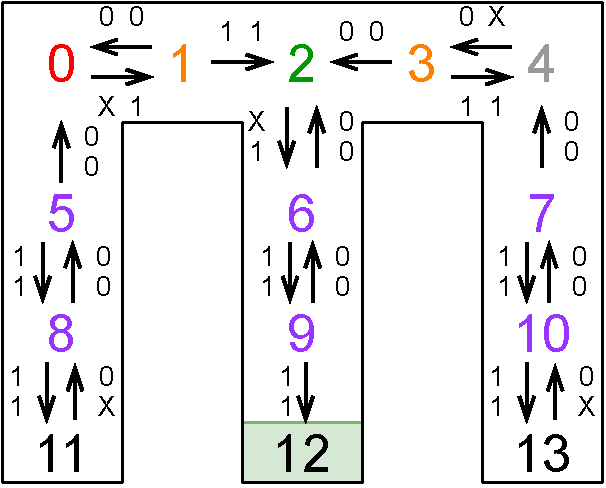
\includegraphics[width=0.4\textwidth]{figures/maze.pdf}
\caption{The state-space of the~\textit{Maze} model with a~marked target state and the~observation groups. A~right side represents the~found optimal strategy to reach the~target location within the~minimal expected time. The~initial state is selected randomly with a~memory value of 0.}%
\label{fig:maze}%
\end{figure}

When an~agent is in the~cell with enclosing walls (cells 0,~2 and 4),~it can navigate to the~exit since it knows its current position within the~maze.
Likewise,~when the~agent navigates from cells $11$ or $13$,~it selects always to the~north to reach cells $0$ or $4$ eventually.
